\documentclass[crop,tikz]{standalone}
\usetikzlibrary{%
    arrows,
    arrows.meta,
    backgrounds,
    calc,
    decorations.pathreplacing,
    fit,
    matrix,
    positioning,
    scopes,
    shadows
}
\usepackage[linguistics]{forest}
\usepackage[charter]{mathdesign}
\tikzset{headarrow/.style = {-{Latex[length=.5em]}}}
\tikzset{move/.style = {dashed,blue,headarrow}}

\newcommand{\mlex}[2]{\ensuremath{\textrm{#1} ::\thinspace \mathrm{#2}}}
\newcommand{\fsel}[1]{\ensuremath{\mathrm{#1^+}}}
\newcommand{\fcat}[1]{\ensuremath{\mathrm{#1^-}}}
\newcommand{\flcr}[1]{\ensuremath{\mathrm{#1^+}}}
\newcommand{\flce}[1]{\ensuremath{\mathrm{#1^-}}}
\newcommand{\fadj}[1]{\ensuremath{\mathrm{#1^\sim}}}
\newcommand{\Merge}{Merge}
\newcommand{\Move}{Move}
\newcommand{\Adjoin}{Adjoin}

\begin{document}
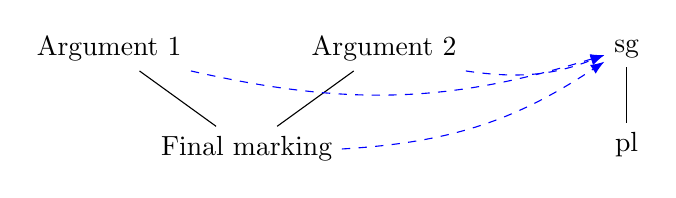
\begin{tikzpicture}
    \node (final) at (0,0) {Final marking};
    \node (arg1) [above left=2em and 2em of final.north] {Argument 1};
    \node (arg2) [above right=2em and 2em of final.north] {Argument 2};

    \node (sg) [right=5em of arg2] {sg};
    \node (pl) [below=2em of sg] {pl};

    \foreach \Source/\Target in {final/arg1, final/arg2, sg/pl}
        \draw (\Source) to (\Target);

    \foreach \Source/\Target in {arg1/sg, arg2/sg, final/sg}
        \draw[move, bend right=15] (\Source) to (\Target);
\end{tikzpicture}
\end{document}
